% interacttfpsample.tex
% v1.01 - June 2016

\documentclass[]{interact}

\usepackage{epstopdf}% To incorporate .eps illustrations using PDFLaTeX, etc.
\usepackage{subfigure}% Support for small, `sub' figures and tables

\usepackage[numbers,sort&compress,merge]{natbib}% Citation support using natbib.sty
\bibpunct[, ]{(}{)}{,}{n}{,}{,}% Citation support using natbib.sty
\renewcommand\bibfont{\fontsize{10}{12}\selectfont}% Bibliography support using natbib.sty
\renewcommand\citenumfont[1]{\textit{#1}}% Citation numbers in italic font using natbib.sty
\renewcommand\bibnumfmt[1]{(#1)}% Parentheses enclose ref. numbers in list using natbib.sty

\theoremstyle{plain}% Theorem-like structures
\newtheorem{theorem}{Theorem}[section]
\newtheorem{lemma}[theorem]{Lemma}
\newtheorem{corollary}[theorem]{Corollary}
\newtheorem{proposition}[theorem]{Proposition}

\theoremstyle{definition}
\newtheorem{definition}[theorem]{Definition}
\newtheorem{example}[theorem]{Example}

\theoremstyle{remark}
\newtheorem{remark}{Remark}
\newtheorem{notation}{Notation}

\begin{document}

\articletype{FINAL PROJECT THESIS}

\title{Fake News Detection Using Deep Learning}

\author{
\name{A.~N. Author\textsuperscript{a}\thanks{CONTACT A.~N. Author. Email: latex.helpdesk@tandf.co.uk} and John Smith\textsuperscript{b}}
\affil{\textsuperscript{a}Taylor \& Francis, 4 Park Square, Milton Park, Abingdon, UK; \textsuperscript{b}Institut f\"{u}r Informatik, Albert-Ludwigs-Universit\"{a}t, Freiburg, Germany}
}

\maketitle

\begin{abstract}
This template is for authors who are preparing a manuscript for a Taylor \& Francis journal using the \LaTeX\ document preparation system and the \texttt{interact} class file, which is available via selected journals' home pages on the Taylor \& Francis website.
\end{abstract}

\begin{keywords}
Sections; lists; figures; tables; mathematics; fonts; references; appendices
\end{keywords}

\section{Introduction}

Lorem ipsum dolor sit amet, consectetur adipiscing elit, sed do eiusmod tempor incididunt ut labore et dolore magna aliqua. Ut enim ad minim veniam, quis nostrud exercitation ullamco laboris nisi ut aliquip ex ea commodo consequat. Duis aute irure dolor in reprehenderit in voluptate velit esse cillum dolore eu fugiat nulla pariatur. Excepteur sint occaecat cupidatat non proident, sunt in culpa qui officia deserunt mollit anim id est laborum.

\section{Related Work}

Lorem ipsum dolor sit amet, consectetur adipiscing elit, sed do eiusmod tempor incididunt ut labore et dolore magna aliqua. Ut enim ad minim veniam, quis nostrud exercitation ullamco laboris nisi ut aliquip ex ea commodo consequat. Duis aute irure dolor in reprehenderit in voluptate velit esse cillum dolore eu fugiat nulla pariatur. Excepteur sint occaecat cupidatat non proident, sunt in culpa qui officia deserunt mollit anim id est laborum.

\subsection{Random Multimodel Deep Learning (RMDL)}

Lorem ipsum dolor sit amet, consectetur adipiscing elit, sed do eiusmod tempor incididunt ut labore et dolore magna aliqua. Ut enim ad minim veniam, quis nostrud exercitation ullamco laboris nisi ut aliquip ex ea commodo consequat. Duis aute irure dolor in reprehenderit in voluptate velit esse cillum dolore eu fugiat nulla pariatur. Excepteur sint occaecat cupidatat non proident, sunt in culpa qui officia deserunt mollit anim id est laborum.


\section{Methodology}

Lorem ipsum dolor sit amet, consectetur adipiscing elit, sed do eiusmod tempor incididunt ut labore et dolore magna aliqua. Ut enim ad minim veniam, quis nostrud exercitation ullamco laboris nisi ut aliquip ex ea commodo consequat. Duis aute irure dolor in reprehenderit in voluptate velit esse cillum dolore eu fugiat nulla pariatur. Excepteur sint occaecat cupidatat non proident, sunt in culpa qui officia deserunt mollit anim id est laborum.

\subsection{Figures}

The \texttt{interact} class file will deal with positioning your figures in the same way as standard \LaTeX. It should not normally be necessary to use the optional \texttt{[htb]} location specifiers of the \texttt{figure} environment in your manuscript, although the \texttt{[p]} option -- i.e.\ \verb"\begin{figure}[p]" -- is useful if you are asked to separate figures from the text.

\begin{figure}[h]
\centering
\subfigure[An example of an individual figure sub-caption.]{
\resizebox*{5cm}{!}{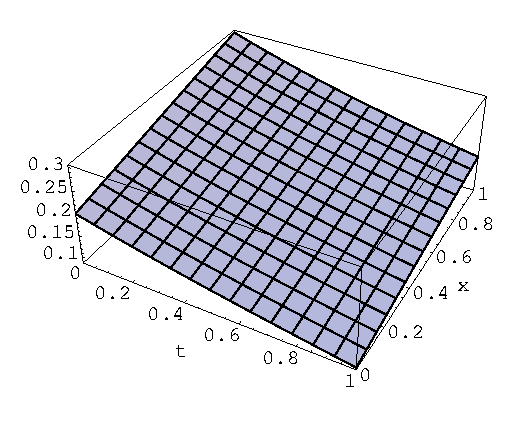
\includegraphics{graph1.eps}}}\hspace{5pt}
\subfigure[A slightly shorter sub-caption.]{
\resizebox*{5cm}{!}{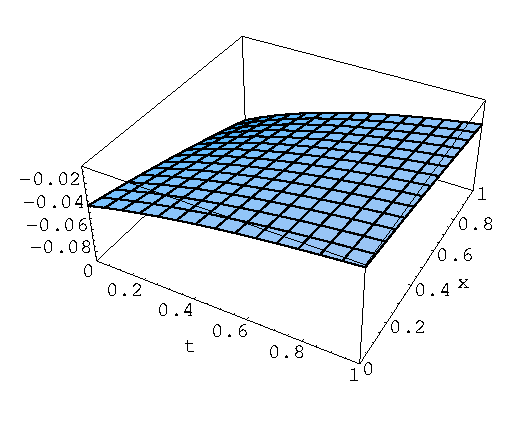
\includegraphics{graph2.eps}}}
\caption{Example of a two-part figure with individual sub-captions
 showing that captions are flush left and justified if greater
 than one line of text.} \label{sample-figure}
\end{figure}

\subsection{Tables}

The \texttt{interact} class file will deal with positioning your tables in the same way as standard \LaTeX. It should not normally be necessary to use the optional \texttt{[htb]} location specifiers of the \texttt{table} environment in your manuscript, although the \texttt{[p]} option -- i.e.\ \verb"\begin{table}[p]" -- is useful if you are asked to separate tables from the text.

\begin{table}[h]
\tbl{Example of a table showing that its caption is as wide as
 the table itself and justified.}
{\begin{tabular}{lcccccc} \toprule
 & \multicolumn{2}{l}{Type} \\ \cmidrule{2-7}
 Class & One & Two & Three & Four & Five & Six \\ \midrule
 Alpha\textsuperscript{a} & A1 & A2 & A3 & A4 & A5 & A6 \\
 Beta & B2 & B2 & B3 & B4 & B5 & B6 \\
 Gamma & C2 & C2 & C3 & C4 & C5 & C6 \\ \bottomrule
\end{tabular}}
\tabnote{\textsuperscript{a}This footnote shows how to include
 footnotes to a table if required.}
\label{sample-table}
\end{table}


\subsection{Mathematics}

\subsubsection{Displayed mathematics}


\begin{equation}
 \hat{\theta}_{w_i} = \hat{\theta}(s(t,\mathcal{U}_{w_i}))
\end{equation}


\section*{Notes}

An unnumbered `Notes' section may be included before the References (if using the \verb"endnotes" package, use the command \verb"\theendnotes" where the notes are to appear, instead of creating a \verb"\section").


\section{References}

\subsection{References cited in the text}

References cited in the text should be quoted by italic numbers in parentheses (e.g.\ (\textit{1}), (\textit{2}, \textit{4}, \textit{10}), (\textit{11}--\textit{15}), \emph{not} (\textit{11})--(\textit{15})), in the order in which they first appear. For further details on this reference style, see the Instructions for Authors on the Taylor \& Francis website.

Each bibliographic entry has a key, which is assigned by the author and used to refer to that entry in the text. In this document, the key \verb"Gou02" in the citation form \verb"\cite{Gou02}" produces `\cite{Gou02}', and the keys \verb"LeC03" and \verb"Ban75" in the citation form \verb"\cite{LeC03,Ban75}" produce `\cite{LeC03,Ban75}'. The citation for a range of bibliographic entries such as `\cite{Sah04,Hil90,Pul04,Kli04,Leo05,Wib74,McG02,Gar88,Zie03,Cha94,Moh04,ACSPD,Car01,Pus05,Mul05,Tay05,Squ05,Len04,Pet99,She04,Tsc04,Cha04}' will automatically be produced by \verb"\cite{Sah04,Hil90,Pul04,Kli04,Leo05,Wib74,McG02,Gar88,Zie03,Cha94,Moh04," \verb"ACSPD,Car01,Pus05,Mul05,Tay05,Squ05,Len04,Pet99,She04,Tsc04,Cha04}". By using the \verb"merge" option to \verb"natbib", citation keys within a multiple \verb"\cite" command may contain a leading \verb"*" that causes them to be merged in the bibliography together with the previous citation as a single entry with a single reference number. For example, \verb"\cite{LP02,*LP04}" produces `\cite{LP02,*LP04}', and both references are listed in the bibliography under one entry with that number.


\subsection{The list of references}

References should be listed at the end of the main text in the order in which they are first cited in the text. Include all author names with surname first, then initials. Separate multiple author names with semicolons, and multiple editor names with commas. If a reference has more than ten authors, list the first ten names followed by `et al.'. The following list shows some sample references prepared in Taylor \& Francis' Reference Style P.

\begin{thebibliography}{99}

\bibitem{Gou02}%01
Gould, S.J. \emph{The Structure of Evolutionary Theory}; Belknap Press:
  Cambridge, MA, 2002.

\bibitem{LeC03}%02
Le~Couteur, P.; Burreson, J. \emph{Napoleon's Buttons: How 17 Molecules Changed
  History}; Jeremy P. Tarcher/Putnam: New York, 2003; pp 32--47.

\bibitem{Ban75}%03
Bandy, A.R., Ed. \emph{The Chemistry of the Atmosphere: Oxidants and Oxidation
  in the Earth's Atmosphere}; Royal Society of Chemistry: Cambridge, UK, 1995.

\bibitem{Sah04}%04
Saha, B.C., Hayashi, K., Eds. \emph{Lignocellulose Biodegradation}; ACS
  Symposium Series 889; American Chemical Society: Washington, DC, 2004.

\bibitem{Hil90}%05
Hillman, L.W. In \emph{Dye Laser Principles with Applications}; Duarte, F.J.,
  Hillman, L.W., Eds.; Academic: New York, 1990; Chapter~2.

\bibitem{Pul04}%06
Puls, J.; Saake, B. Industrially Isolated Hemicelluloses. In
  \emph{Hemicelluloses: Science and Technology}; Gatenholm, P., Tenkanen, M.,
  Eds.; ACS Symposium Series 864; American Chemical Society: Washington, DC,
  2004; pp 24--37.

\bibitem{Kli04}%07
Kline, R.B. \emph{Principles and Practice of Structural Equation Modeling}, 2nd
  ed.; Guilford Press: New York, 2004.

\bibitem{Leo05}%08
Leone, S.R., McDermott, A.E., Paul, A., Eds. \emph{Annual Review of Physical
  Chemistry}; Annual Reviews: Palo Alto, CA, 2005; Vol.~56.

\bibitem{Wib74}%09
Wiberg, K. In \emph{Investigations of Rates and Mechanisms of Reactions};
  Lewis, E.S., Ed.; Techniques of Chemistry, Vol.~VI, Part~I; Wiley: New York,
  1974; p 764.

\bibitem{McG02}%10
\emph{McGraw-Hill Encyclopedia of Science and Technology}, 9th ed.;
  McGraw-Hill: New York, 2002; 20 vols.

\bibitem{Gar88}%11
Garrone, E.; Ugliengo, P. In \emph{Structure and Reactivity of Surfaces},
  Proceedings of the European Conference, Trieste, Italy, Sept~13--20, 1988;
  Zecchina, A., Cost, G., Morterra, C., Eds.; Elsevier: Amsterdam, 1988.

\bibitem{Zie03}%12
Zientek, K.D.; Eyler, J.R. Presented at the 51st ASMS Conference on Mass
  Spectrometry and Allied Topics, Montreal, Canada, June~8--12, 2003.

\bibitem{Cha94}%13
Chandrakanth, J.S. Effects of Ozone on the Colloidal Stability of Particles
  Coated with Natural Organic Matter. Ph.D. Dissertation, University of
  Colorado, Boulder, CO, 1994.

\bibitem{Moh04}%14
Mohamed, M. Waterjet Cutting Up to 900~MPa. Ph.D. Thesis, University of
  Hannover, Germany, 2004.

\bibitem{ACSPD}%15
ACS Publications Division Home Page. http://pubs.acs.org (accessed Nov~7,
  2004).

\bibitem{Car01}%16
Caruso, R.A.; Susha, A.; Caruso, F. Multilayered Titania, Silica and Laponite 
  Nanoparticle Coatings on Polystyrene Colloidal Templates. \emph{Chem. Mater.} 
  \textbf{2001}, \emph{13}, 400--409.

\bibitem{Pus05}%17
Puskas, J.E.; Chan, S.W.P.; McAuley, K.B.; Shaikh, S.; Kaszas, G. \emph{J.
  Polym. Sci., Part A: Polym. Chem.} \textbf{2005}, \emph{43}, 5394--5413 and
  references therein.

\bibitem{Mul05}%18
Mullin, R. \emph{Chem. Eng. News} \textbf{2005}, \emph{83}~(Oct~17), 7.

\bibitem{Tay05}%19
Taylor, C.W.; Kumar, S. \emph{Eur. J. Cancer} \textbf{2005},
  \emph{40}~(Suppl.~1), 781.

\bibitem{Squ05}%20
Squires, S. Falling Short on Nutrients. \emph{The Washington Post}, Oct~4,
  2005, p H1.

\bibitem{Len04}%21
Lenssen, K.C.; Jantscheff, P.; Kiedrowski, G.; Massing, U. Cationic Lipids with
  Serine Backbone for Transfecting Biological Molecules. Eur. Pat. Appl.
  1457483, 2004.

\bibitem{Pet99}%22
Petrovick, P.R.; Carlini, E. Antiulcerogenic Preparation from \emph{Maytenus
  ilicifolia} and Obtaintion Process. Br. Patent PI 994502, March~6, 1999.

\bibitem{She04}%23
Sheem, S.K. Low-Cost Fiber Optic Pressure Sensor. US Patent 6,738,537,
  May~18, 2004.

\bibitem{Tsc04}%24
Tschantz, B.A.; Moran, B.M. \emph{Modeling of the Hydrologic Transport of
  Mercury in the UEFPC Watershed}; Technical Report for Lockheed Martin Energy 
  Systems: Bethesda, MD, September 2004.

\bibitem{Cha04}%25
Chatterjee, K.; Visconti, A.; Mirocha, C.J. Deepoxy T-2 Tetraol: A Metabolite
  of T-2 Toxin Found in Cow Urine. \emph{J. Agric. Food Chem.}, submitted for
  publication, 2004.

\bibitem{LP02}%26a
Lu, Y.; Pignatello, J.J. \emph{Environ. Sci. Technol.} \textbf{2002},
  \emph{36}, 4553--4561.

\bibitem{LP04}%26b
Lu, Y.; Pignatello, J.J. \emph{Environ. Sci. Technol.} \textbf{2004},
  \emph{38}, 5853--5862.

\end{thebibliography}
\bigskip

\bigskip


\section{Appendices}

\appendix
\section{Troubleshooting}

Authors may occasionally encounter problems with the preparation of a manuscript using \LaTeX. The appropriate action to take will depend on the nature of the problem:
\begin{enumerate}
\item[(i)] If the problem is with \LaTeX\ itself, rather than with the actual macros, please consult an appropriate \LaTeXe\ manual for initial advice. If the solution cannot be found, or if you suspect that the problem does lie with the macros, then please contact Taylor \& Francis for assistance (\texttt{latex.helpdesk@tandf.co.uk}).
\item[(ii)] Problems with page make-up (e.g.\ occasional overlong lines of text; figures or tables appearing out of order): please do not try to fix these using `hard' page make-up commands -- the typesetter will deal with such problems. (You may, if you wish, draw attention to particular problems when submitting the final version of your manuscript.)
\item[(iii)] If a required font is not available on your system, allow \TeX\ to substitute the font and specify which font is required in a covering letter accompanying your files.
\end{enumerate}


\section{Obtaining the template and class file}

\subsection{Via the Taylor \& Francis website}

This article template and the \texttt{interact} class file may be obtained via the `Instructions for Authors' pages of selected Taylor \& Francis journals.

Please note that the class file calls up the open-source \LaTeX\ packages booktabs.sty, epsfig.sty and rotating.sty, which will, for convenience, unpack with the downloaded template and class file. The template calls for natbib.sty and subfigure.sty, which are also supplied for convenience.


\subsection{Via e-mail}

This article template, the \texttt{interact} class file and the associated open-source \LaTeX\ packages are also available via e-mail. Requests should be addressed to \texttt{latex.helpdesk@tandf.co.uk}, clearly stating for which journal you require the template and class file.

\end{document}
